\documentclass[11pt, letterpaper]{article}

\usepackage[margin=1in]{geometry}
\usepackage{setspace}
\onehalfspacing
\usepackage{authblk}
\usepackage{mathtools}
\usepackage{amsmath, amsfonts, amssymb}
\usepackage{booktabs}
\usepackage{cite}
\usepackage{hyperref}
\usepackage{dsfont}
\usepackage[section]{placeins}
\usepackage{pgfplots}
\pgfplotsset{compat=1.18}
\usepackage{subcaption}
\usepackage{graphicx}
\usepgfplotslibrary{groupplots}

\newcommand{\sfw}{0.30\textwidth}

\pgfplotsset{
    gammascale/.style={
        scaled y ticks=false,
        yticklabel={
            \pgfmathparse{\tick*100}%
            \pgfmathprintnumber[
                fixed,
                precision=1
            ]{\pgfmathresult}
        },
        ylabel={$\gamma\ (\times 10^{-2})$},
    }
  }

\pgfplotsset{
    my3dsurf/.style={
        width=\linewidth,
        height=5cm,
        font=\small,
        tick label style={font=\tiny},
        label style={font=\scriptsize},
        view={-50}{28},
        colormap/viridis,
        grid=major,
    }
}

\newlength{\figgap}\setlength{\figgap}{2.4cm}
\newcommand{\panelw}{0.40\textwidth}
\usepackage{titlesec}
\hypersetup{
    colorlinks=true,
    linkcolor=black,
    filecolor=black,
    urlcolor=blue,
    citecolor=black
}

\definecolor{codegreen}{rgb}{0,0.6,0}
\definecolor{codegray}{rgb}{0.5,0.5,0.5}
\definecolor{codepurple}{rgb}{0.58,0,0.82}
\definecolor{backcolour}{rgb}{0.98,0.98,0.98}
\allowdisplaybreaks

\title{Penalized Portfolio Optimization}
\author{Victor Ding}
\affil{New Canaan High School}
\date{\today}


\begin{document}

\maketitle
\thispagestyle{empty}
\newpage

\begin{abstract}
  \thispagestyle{empty}
  \noindent
This research reviews practical considerations of long-short portfolio optimization problems. It studies a few penalty forms to
address the limitations of pure constraints.

The Alpha Gate penalizes excess turnover above a soft threshold, with a higher hard bound acting as a strict
safeguard. Regularization penalties widely used in regression are adapted to prune noisy trades. Elastic Net and the Berhu
function both use \(L_1\) and \(L_2\) penalties on turnovers, but differently: Elastic Net keeps both active at every trade
size, whereas Berhu applies \(L_1\) below a threshold and \(L_2\) above it.

We run various experiments with these penalties on ten years of daily long-short equity signals, evaluating turnover control,
target-tracking loss, and trade sparsity across parameter ranges.
\end{abstract}

\newpage
\pagestyle{plain}
\setcounter{page}{1}

\section{Introduction}
Modern portfolio construction is fundamentally an optimization problem. Typically, a starting portfolio of existing positions is
adjusted to a final portfolio. Position limits, attribute-exposure limits, and turnover budgets are standard constraints in
quantitative portfolio management.

Since each constraint shrinks the feasible set of solutions, proliferating constraints can leave only a tiny feasible
region. This problem is amplified by estimation error and data noise in the model inputs. Hard constraints alone are therefore
overly rigid and often unsatisfactory.

This paper primarily studies penalty mechanisms for softening these rigidities. Our research proceeds as follows. We outline the
framework in Section \ref{sec:framework}, where we review the various technicalities and practicalities of
constrained portfolio optimization. We formalize the Alpha Gate as a soft turnover cap in Section \ref{sec:alpha_gate}.  Section
\ref{sec:regularization} covers Elastic Net and Berhu penalties used to prune noisy trades. In Section \ref{sec:experiments},
we use numerical experiments to illustrate the features and effectiveness of these penalty forms. Along the way, we
also discuss the considerations for the choice of various penalty parameters. We highlight some important outstanding issues for
future research in Section \ref{sec:conclusion}.

\section{Implementation Framework}
\label{sec:framework}

This section sets out the theoretical framework used in the remainder of the paper. We lay out the optimization problem with all
the common constraints on long-short portfolios. We also discuss the techniques for handling non-differentiability and
non-convexity.

\subsection{Objective Functions and Convexity}
Modern portfolio construction involves optimizing an objective function defined over a vector of $n$ asset positions
$w \in \mathds{R}^n$, where positive (negative) values represent long (short) positions. An example of a classic objective
function is Markowitz's Mean-Variance framework:
\begin{equation}
    \label{mean-variance_objective}
    \underset{w}{\min} \left[\frac{\lambda}{2} w^\top \Sigma w - r^\top w\right],
\end{equation}
where $r$ is a vector of expected returns, $\lambda$ is an exogenous risk-aversion parameter, and $\Sigma$ is a covariance
matrix of asset returns. The design is driven by the desire to strike a balance between risks and payoffs.

Objective functions can take other forms, such as the squared $L_2$ from a target vector $\tilde{w} \in
\mathds{R}^n$. A given vector $\tilde{w}$ can be a benchmark portfolio to track, or a target portfolio driven by some
forecasting models. It is often desirable to mimic such a portfolio as closely as possible. One reasonable approach is to
minimize this objective:
\begin{equation}
  \label{eq:simple_tracking}
	\underset{w}{\min} \lVert w - \tilde{w}\rVert_2^2.
\end{equation}
A positive semi-definite covariance matrix $\Gamma$ can also be incorporated to generalize the above objective function further:
\begin{equation}
  \label{gamma_matrix}
	\underset{w}{\min}\left[\frac{1}{2} (w - \tilde{w})^\top\Gamma(w - \tilde{w})\right] =
  \underset{w}{\min}\left[\frac{1}{2} w^\top\Gamma w - \tilde{w}^\top\Gamma w \right].
\end{equation}
Mathematically, this expression is a special case of \eqref{mean-variance_objective}.

A majority of portfolio construction problems can be formulated as optimizing certain quadratic forms like the above subject to
some linear constraints. While potential payoffs are often uncertain, transaction costs are incurred upon execution. Turnover
budgets and individual turnovers are often imposed, so a solution is discouraged from chasing marginal benefits with excessive
transaction costs. Other typical constraints include limit on risk exposures.

Objective function \eqref{mean-variance_objective} is convex if $\Sigma$ is positive semi-definite. The optimization problem of
such an objective function has a global optimal solution if the constraints also maintain a convex feasible set.

Let us focus on minimizing the family of objectives with a quadratic term $q(w)$, which captures the conventional Mean-Variance
problem \eqref{mean-variance_objective} and target tracking problem \eqref{gamma_matrix}. Such objectives are within the reach
of Disciplined Convex Programming (DCP). DCP problems can be easily solved with DCP solvers.

Linear equalities, and inequalities define hyperplanes and half-spaces respectively. Half-spaces, along with second-order cones,
define convex sets. Hyperplanes are affine, and thus convex sets. When feasible sets are convex, optimization is often far more
efficient and accurate. Because of this, we show a preference for preserving convexity of the overall feasible region. For
constraints that are non-smooth but inherently convex (such as absolute value or piecewise functions), we use exact epigraph
reformulations with auxiliary variables. For constraints that are truly non-convex, we employ convex restrictions to approximate
the feasible space while maintaining computational tractability.

\subsection{Constraints}
Inputs such as return estimates, risk model coefficients, and target forecasts in $\tilde{w}$ are all estimates subject to
estimation errors and data noise. Thus, a problem subject to overly permissive constraints is susceptible to concentrated
positions with potentially poor signals. On the other hand, we also look to avoid overly tight constraints. While constraints
have their purposes and those like turnover and position limits may even serve as a natural form of regularization on model
solutions, each one shrinks the feasible set of potential solutions. Tight constraints may force solutions that reflect little
of their intended objective functions. Ideally, constraints should be set such that they do not ''drive'' the solution; instead a
solution should be dictated primarily by the objective function.

Hard constraints that bound turnover and other portfolio characteristics have certain downsides. We prefer to impose them to
reflect practical and risk limits, rather than determining optimality. Violating a hard constraint by a negligible amount and by a
comparatively huge amount has the same effect, meaning rounding errors, tiny violations, and genuine infeasibility are
treated equally. Furthermore, some powerful signals may warrant trading significantly more, either of individual assets or
across the entire portfolio when the risk-adjusted payoffs far exceed the likely incurred transaction costs. In those cases, it is
desirable to permit certain violations of hard constraints. To achieve this, we introduce soft constraints.

Soft constraints allow breaches of some thresholds while discouraging large ones by adding a penalty to the objective function. We
will consider three distinct types of soft constraints: a turnover penalty, an Elastic Net, and a Berhu penalty.

Position limits can be represented as
\begin{align*}
    \underline{w} & \leq w \leq \overline{w},
\end{align*}
where constant vectors $\underline{w} \in \mathds{R}^n$ and $\overline{w} \in \mathds{R}^n$ are lower and upper bounds, respectively.

Similarly, limits on each individual turnover are represented by $|w - w^*| \leq t$, where constant $t \in \mathds{R}^n$ defines
individual turnover bounds, and $w^*$ represents the starting weight vector. Turnover bounds can be essentially incorporated
into position limits because $w^*$ is a constant vector.

We define an attribute as a characteristic of an asset. It is common to cap portfolio exposures to sectors and
industries. Equity style factors (growth, momentum, value, etc.) are also types of attributes widely used in risk modeling. An
asset can have exposures to multiple attributes. For example, although a small tech startup can have exposure to just the
technology sector, a conglomerate operates in several. Attribute exposures can also be negative. Smaller companies, for example,
tend to have negative exposures to size factors.

We express $n$ assets' exposure in $m$ attributes with an $m\times n$ matrix $\mathbf{S}$. A hypothetical $\mathbf{S}$ for $n$
assets across various attributes is shown in Table \ref{example_attribute_matrix}.  The total portfolio exposures to the $m$
factors are $\mathbf{S}w$. The exposure limits can be represented as
\begin{equation}
    \underline{s} \leq \mathbf{S}w \leq \overline{s},
\end{equation}
where $\underline{s}$ and $\overline{s}$ are lower and upper exposure bounds, respectively.

\begin{table}[t]
\centering
\caption{Example Factor Loading Matrix.}
\label{example_attribute_matrix}
    \vspace{0.3cm}
    \begin{tabular}{cr *{5}{c}}
        \toprule
        & & \multicolumn{5}{c}{\textbf{Assets}} \\
        \cmidrule(lr){3-7}
        & & \textbf{1} & \textbf{2} & \textbf{3} & \dots & \textbf{$n$} \\
        \cmidrule(lr){1-7}
        & Finance & 0.10 & 0.40 & 0.20 & \dots & $A_n$ \\
        & Energy & 0.13 & 0.20 & 0.30 & \dots & $B_n$ \\
        & Communication & 0.06 & 0.04 & 0.10 & \dots & $C_n$ \\
        & \dots & \dots & \dots & \dots & \dots & \dots \\
        \cmidrule(lr){1-7}
        & Growth & 0.70 & 0.30 & 0.20 & \dots & $D_n$ \\
        & Momentum & -1.0 & -0.30 & 0.10 & \dots & $E_n$ \\
        & \dots & \dots & \dots & \dots & \dots & \dots \\
        \bottomrule
    \end{tabular}
\end{table}

Net exposure, equal to the value of long positions minus the value of short positions, is a special form of attributes. It can
be captured as a row of ones in $\mathbf{S}$.

A constant upper bound $T > 0$ may be imposed on total turnover as
\begin{equation}
    \label{unedited_total_turnover}
	\lVert w^* - w\rVert_1 \leq T.
\end{equation}
This introduces a total budget over the sum of individual turnovers. In practice, individual turnover limits $t$ are often set
such that $T < \sum_i t_i$; otherwise, the total turnover cap will become redundant. Total turnover can be further
generalized with a weighting vector $c > 0$ such that
\begin{equation}\label{eq:tvr-tight}
	c^\top |w^* - w| \leq T.
\end{equation}
The vector $c$ and $T$ may represent some transaction cost estimates and a budget limit, respectively. When turnovers are
equally weighted, constraint \eqref{eq:tvr-tight} becomes \eqref{unedited_total_turnover}.

The constraint \eqref{unedited_total_turnover} or \eqref{eq:tvr-tight} is not directly supported by many solvers. Although
convex, it is not affine, and is not differentiable at $w^*$. We introduce the slack vector $f \in \mathds{R}^n$, such that
\begin{equation}\label{eq:tvr-slack}
	|w^* - w| \leq f, \quad c^\top f \leq T.
\end{equation}
A feasible $f$ exists if and only if $c^\top |w^* - w| \leq T$. Hence, \eqref{eq:tvr-slack} and \eqref{eq:tvr-tight} define the
same feasible set of $w$.

Gross exposure, $\lvert w\rVert_1$, is another measure often involved in some constraints, as it is often desirable to keep a
specific amount of capital invested in a portfolio. It is common to limit the gross exposure (leverage) by an upper bound $G$ as
\begin{equation}\label{eq:exposure-ineq}
	\lVert w\rVert_1 \leq G.
\end{equation}
This is still a convex constraint like that on total turnovers. But the optimal solution may find it cheaper to settle at a
gross exposure far less than $G$, effectively underinvesting with available capital. It is thus attractive to place a lower
bound $\underline{G}$ on the gross exposure as well. When $G=\underline{G}$, the constraint becomes an equality
\begin{equation}
    \label{explicit_gross_exposure}
	\lVert w\rVert_1 = G.
\end{equation}
In long-only or short-only portfolios, absolute value signs in \eqref{explicit_gross_exposure} can be trivially removed so that
it becomes a convex constraint. But the presence of a lower bound or equality constraints in long-short portfolios makes the
feasible set non-convex, which poses a problem for most solvers. We will address this non-convexity in section
\ref{gross_exposure_section}.

\subsection{Global Optimality Conditions and Difficulties of Gross Exposure}
\label{gross_exposure_section}
Suppose a quadratic objective is bounded by affine constraints that create a convex feasible set. The Karush-Kuhn-Tucker (KKT)
conditions \cite{boyd2004KKT} define the framework for determining optimality.

In an optimization setting with quadratic objective function, a positive semi-definite Hessian matrix ensures the convexity of
the objective. When constraints are affine, the feasible set is also convex. Under such conditions, a local optimal minimum is
also the global minimum and its solution can be calculated via DCP.

A well-behaved covariance matrix $\Sigma$ in \eqref{mean-variance_objective} is positive semi-definite, so is $\Gamma$ in
\eqref{gamma_matrix}. Almost all the constraints discussed so far are also convex except for gross exposure.

A set $\mathcal{C} \subset \mathds{R}^n$ is convex if and only if for any two points $a$ and $b$ in $\mathcal{C}$ and every
$\theta \in [0,1]$ the following is true:
\begin{equation}
	\theta a + (1 - \theta)b \in \mathcal{C}.
\end{equation}
We will prove that for a fixed $G > 0$, the set $\mathcal{S} = \{w\in \mathds{R}^n:\lVert w\rVert_1 = G\}$ is not convex.  This
argument does not restrict itself to properties of the $L_1$ norm. Rather, it uses two axioms every norm satisfies:
\begin{enumerate}
	\item Absolute Homogeneity: $\lVert\alpha w\rVert = |\alpha| \lVert w\rVert$ for any scalar $\alpha$.
	\item Positive definiteness: $\lVert w\rVert = 0 \Leftrightarrow w = 0$.
\end{enumerate}
Take any $w \in \mathcal{S}$. By homogeneity with $\alpha = -1$, we have
\begin{equation*}
	\lVert-w\rVert_1 = | -1|\cdot \lVert w\rVert_1 = \lVert w\rVert_1 = G.
\end{equation*}
This implies $-w \in \mathcal{S}$. For $\theta = \frac{1}{2}$, we have $\theta w + (1-\theta)(-w) = 0 \notin
\mathcal{S}$. Therefore, the set $\mathcal{S}$ is not convex.

The non-convexity arises from the uncertain signs of the optimal solution, which are not known prior to the solution process. We
can rewrite $w$ as $w^+-w^-$, where both $w^+$ and $w^-$ are nonnegative vectors in $\mathds{R}^n$. This allows us to represent
$G$ as $e^\top(w^++w^-)$. The problem is that $w_i^+w_i^-$ must equal $0$ for all $i$ or a solver will freely choose them to hit
the target $G$. Even Mixed-Integer Convex Programming (MICP) will have difficulty finding an optimal solution in a timely and
resource-efficient manner when $n$ is reasonably large.

One way to overcome this is forcing the signs of $\{w_i\}$ according to some rules prior to setting up the gross exposure
constraint. Let $G^+ > 0$ be the desired long exposure, and $G^- < 0$ be the negative counterpart. The total gross exposure
becomes $G^+ - G^- = G$. For tracking problems of \eqref{gamma_matrix}, we propose to match the sign of $w$ to that of
$\tilde{w}$ such that
\begin{equation}
  \label{eq:gross_exposure}
  \begin{aligned}
    w_i \geq 0, \quad & \forall i\in\mathcal{W}^+ := \{i \mid \tilde{w}_i > 0\} ,\\
    w_i \leq 0, \quad & \forall i\in\mathcal{W}^- := \{i \mid \tilde{w}_i < 0\} ,\\
    w_i = 0, \quad & \forall i\in\mathcal{W}^0 := \{i \mid \tilde{w}_i = 0\}.
  \end{aligned}
\end{equation}
Furthermore, we require that
\begin{equation*}
	\sum_{i\in\mathcal{W}^+}w_i = G^+, \quad \sum_{i\in\mathcal{W}^-}w_i = G^-.
\end{equation*}
The price is that the feasible set is effectively shrunk, and consequently may not yield the same global optimal solution of
the original problem.

Other local search methods may improve upon this approach:
\begin{itemize}
\item Solve the original problem with inequality \eqref{eq:exposure-ineq}, and use the signs of the solution vector to derive
  $\mathcal{W}^+$, $\mathcal{W}^-$, and $\mathcal{W}^0$. Solve the problem with the equality constraint along with the
  determined signs.
\item After one iteration, flip the signs of assets with $|w_i|$ inside a small band $\epsilon$ to update $\mathcal{W}^+$,
  $\mathcal{W}^-$, and $\mathcal{W}^0$. Solve again. If there is improvement, increase $\epsilon$ and repeat.  If not, stop.
\item Solve the original problem with inequality \eqref{eq:exposure-ineq}, and scale all the weights such that
  $\lVert w\rVert_1 = G$.  Feed the results back to iterate.
\item An approach in the same spirit as the penalty forms discussed later is to introduce a slack variable $g \geq 0$ such that
  $\lVert w\rVert_1 + g = G$, and a penalty term $\eta g$. A sufficiently large parameter $\eta$ will cause $g$ to be 0 at
  the optimal solution. Fix the signs according to the solutions of this penalized optimization and solve the original problem
  without the penalty term.
\end{itemize}
Unfortunately, these are all heuristic approaches to resolve sign uncertainty prior to the optimization. None of these
approaches can guarantee the global optimum. As long as the feasible set is not expanded like \eqref{eq:exposure-ineq}, the
objective functions across various heuristic approaches can be compared to each other to evaluate the improvement of each step.

\section{Hard and Soft Caps of Transaction Costs}
\label{sec:alpha_gate}

Trading from $w^*$ to $w$ incurs transaction costs. It is thus desirable to balance the objective function and turnover to
avoid paying deterministic upfront costs for insignificant or uncertain transactions. Imposing a hard budget limit on total
turnover, however, handicaps portfolio construction from achieving its objective. Instead, we should explore the potential
trade-offs of excessive turnovers.

In addition to a hard upper bound $T$ on total turnover \eqref{unedited_total_turnover} or as its replacement, we introduce a
slack variable $z \geq 0$ to relax a constant soft bound $\tilde{T} > 0$ such that
\begin{equation*}
	\lVert w - w^*\rVert_1 \leq \tilde{T} + z,
\end{equation*}
and add a penalty term to the objective function $q(\cdot)$,
\begin{equation}\label{eq:tvr-total}
	p(z) = \alpha z^2.
\end{equation}
This term will be referred to as Alpha Gate. The exogenous parameter $\alpha > 0$ determines the cost of going above
$\tilde{T}$. The variable $z$ will be optimized along with $w$. The quadratic term has the benefit of having a comparable
magnitude with many objective function forms of $q(w)$ such that the choice of $\alpha$ is more intuitive. It is completely
reasonable to replace it with $\alpha |z|$. The presence of an absolute value poses no technical difficulty here given that
$z \geq 0$.

This formulation is very intuitive. The total turnover is allowed to exceed $\tilde{T}$, but pays a penalty to do so. If
turnover is less than $\tilde{T}$, no penalty is paid. The larger the value of $\alpha$, the more strongly the total turnover is
discouraged from exceeding $\tilde{T}$, and vice versa. This ``soft cap'' is not a rigid hard bound, allowing some room to trade more
when situation dictates it. When both a ``hard cap'' and a ``soft cap'' are present, we generally have $\tilde{T} < T$ in that
$T$ serves as a rigid safeguard on the total turnover.

\section{Regularization of Noisy Trades}
\label{sec:regularization}

While individual turnover and transaction budget constraints are common in portfolio construction, it is also desirable to
reduce the number of inconsequential small trades. They are either results of some computational or statistical noises, or are
simply too insignificant to justify the execution or handling costs. Eliminating such small trades also gives the turnover
budget to other assets.

We wish to induce a degree of sparsity in a portfolio's turnovers, pruning noisy trades. A popular method to encourage sparsity
involves setting a certain threshold for $\lvert w_i - w^*_i \rvert$, below which those $\{w_i\}$ will be forced to stay at
$\{w_i^*\}$, meaning no trade allowed. However, this ad-hoc rule may be too rigid, and the threshold setting also seems rather
arbitrary.

This problem is very similar to variable selection in various regression frameworks where coefficients of some variables are
shrunk towards zero to yield parsimonious models. It is thus not surprising that similar techniques can be employed to
regularize $|w - w^*|$.

\subsection{Elastic Net}

Ridge Regression \cite{hoerl1970ridge} softens estimated coefficients through a scaled $L_2$ norm. Lasso regression
\cite{tibshirani1996lasso} utilizes an $L_1$ norm instead. The Elastic Net \cite{zou2005elasticnet} uses both $L_1$ and $L_2$
norms simultaneously. This concept can be adopted for portfolio optimization, penalizing turnovers:
\begin{equation}
	\label{elastic_net_objective}
	\gamma\left[\beta \lVert w-w^*\rVert_1 + \frac{1 - \beta}{2} \lVert w-w^*\rVert_2^2\right],
\end{equation}
where $0 \leq \beta \leq 1$ and $\gamma > 0$ are adjustable exogenous parameters. It can be added to a base quadratic objective
$q(\cdot)$ along with other penalty terms such as \eqref{eq:tvr-total}.  Each term in the objective is either an $L_1$ norm,
$L_2$ norm, or a quadratic function. Since all scalars $\alpha$, $\beta$, and $\gamma$ are positive, the entire objective
function maintains its convexity.

The $L_1$ penalty promotes sparsity, driving small turnovers to $0$. The $L_2$ penalty promotes smoothness. It prevents related
trades from swinging violently with tiny input changes. Turnovers among correlated assets are distributed more evenly than with
only an $L_1$ penalty. For example, the $L_2$ penalty resulting from two turnovers $0.2$ and $0.2$ is smaller than the penalty
resulting from $0.1$ and $0.3$, even though the total turnover is the same. The parameter $\beta$ governs relative strength of
penalties between the two terms.

The parameter $\gamma$ controls the overall scale of this penalty term relative to the objective function $q(\cdot)$.  A larger
$\gamma\beta$ reflects a higher marginal cost of initiating a new trade, pushing some small trades towards zero.

\subsection{Berhu (Reverse Huber) Loss}
Elastic Net penalties in the last section subject trades to both $L_1$ and $L_2$ penalties, regardless of the magnitude of a
trade. It tends to reduce turnovers indiscriminately. The Berhu (Reverse Huber) loss \cite{owen2007robust} is a piecewise
function that contains either an $L_1$ or $L_2$ penalty over non-overlapping regions.

Frequently used in regressions, the Huber's loss function of $q_i$ with a threshold scalar $\epsilon > 0$ takes the form
\begin{equation}
  h(q_i) = \begin{cases}
    \frac{q_i^2}{2\epsilon}, & |q_i| \leq \epsilon, \\
    |q_i| - \frac{\epsilon}{2}, & |q_i| > \epsilon.
  \end{cases}
\end{equation}
It applies a quadratic penalty for small deviations, and a linear penalty for large deviations. This dampens the influence of
extreme outliers in regression while maintaining differentiability throughout. It can serve as a drop-in replacement for the
$L_2$ loss function \eqref{eq:simple_tracking}. Because of reduced responses to large deviations, it may reduce the incentive to
match extreme target positions aggressively, which in some cases may also lead to lower turnovers.

Berhu Loss, also known as Reverse Huber's loss, inverts the order of the quadratic and linear functions. Given
$y_i = w_i - w_i^*$, the Berhu Loss is defined as
\begin{equation}
  \label{berhu_func}
  b(y_i) = \begin{cases}
    |y_i|, & |y_i| \leq \epsilon, \\
    \frac{y_i^2 + \epsilon^2}{2\epsilon}, & |y_i| > \epsilon.
  \end{cases}
\end{equation}

The Berhu function works similarly to Elastic Net, but only applies either an $L_1$ norm or $L_2$ norm at a time. For minor
weight adjustments where $|y_i| \leq \epsilon$, the penalty is linear, promoting sparsity. For significant weight adjustments
where $|y_i| \geq \epsilon$, the penalty becomes quadratic and tend to spread trades across assets.

Intuitively, both Elastic Net and Berhu function preserve non-differentiable vertices, which provide opportunities for some
$\{y_i\}$ to drop to zero. An Elastic Net also adds curved edges that offer surfaces for the loss contour to settle where highly
correlated ones are involved. The Berhu function shrinks the areas of straight edges. Both encourage more control variables to
go towards zero upon contact with the objective contour at the optimal solution, just in slightly different fashions. Once a
turnover exceeds $\epsilon$, the Berhu Loss becomes quadratic while the Elastic Net still maintains an $L_1$ term. In the
parameter range studied here where $\epsilon \ll 1$, this quadratic term is larger than the quadratic term of the Elastic Net
with the same $\gamma$. This comparison is parameter dependent in general. A properly chosen $\epsilon$ can apply $L_1$ penalty
to some trades while subjecting the rest to $L_2$ penalty.

One advantage that Elastic Net maintains over the Berhu function is in its handling of correlated trades. Since only $L_1$
penalty is effective for the trade magnitudes below $\epsilon$, the Berhu shrinkage is highly sensitive to correlated trades
whose magnitudes are also below $\epsilon$, just like Lasso is over such reduced space. It, however, may not be a serious issue
because the affected trades must be highly correlated and at the same time have magnitudes less than $\epsilon$.

\begin{figure}
	\centering

	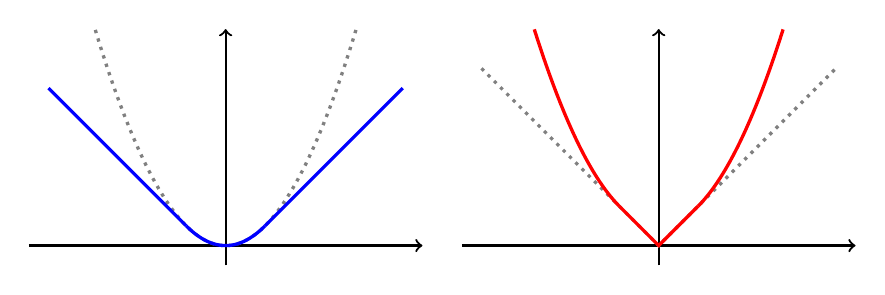
\begin{tikzpicture}[scale=0.5, transform shape]

    %Huber's Function
    \begin{scope}[xshift=-5.5cm]
        %Axes
        \draw[->, thick] (-5, 0) -- (5, 0);
        \draw[->, thick] (0, -0.5) -- (0, 5.5);

        % extension
        \draw[gray, very thick, dotted, domain=-3.31:3.31, samples=100] plot (\x, {0.5*\x*\x});

        % Huber function (blue)
        \draw[blue, very thick] (-4.5, 4) -- (-1, 0.5);
        \draw[blue, very thick, domain=-1:1, samples=50] plot (\x, {0.5*\x*\x});
        \draw[blue, very thick] (1, 0.5) -- (4.5, 4);
    \end{scope}

    %Berhu Function
    \begin{scope}[xshift=5.5cm]
        %Axes
        \draw[->, thick] (-5, 0) -- (5, 0);
        \draw[->, thick] (0, -0.5) -- (0, 5.5);

        % extension
        \draw[gray, very thick, dotted] (-4.5, 4.5) -- (0, 0) -- (4.5, 4.5);

        % Berhu function (Red)
        \draw[red, very thick, domain=-3.16:-1, samples=50] plot (\x, {0.5*(\x*\x + 1)});
        \draw[red, very thick] (-1, 1) -- (0, 0) -- (1, 1);
        \draw[red, very thick, domain=1:3.16, samples=50] plot (\x, {0.5*(\x*\x + 1)});
    \end{scope}
    \end{tikzpicture}
    \caption{Huber's Loss (Left) and Berhu Loss (Right)}
\end{figure}
The Berhu function is convex and continuous everywhere. That said, its piecewise nature makes it difficult to implement
directly into a solver, as many solvers do not accept piecewise functions natively or have a designated Berhu function.
To resolve this, we will create an epigraph formulation with auxiliary variables.

Define two non-negative vectors $u \geq 0$ and $v \geq 0$ subject to the following constraints for all $i$:
\begin{equation*}
	u_i + v_i \geq |y_i|, \quad u_i \leq \epsilon.
\end{equation*}
The Berhu Loss then becomes
\begin{equation}
  \label{berhu_epigraph}
	b(y) = \sum_i \left(u_i + v_i + \frac{v_i^2}{2\epsilon}\right).
\end{equation}
When $|y_i| \leq \epsilon$, to minimize the penalty, the solver will set $v_i = 0$ because the quadratic penalty term
$\frac{v_i^2}{2\epsilon}$ grows more rapidly than the linear term $u_i$, being more ``expensive'' in the objective function. The
constraint $u_i + v_i \geq |y_i|$ forces $u_i = |y_i|$, making the penalty exactly $|y_i|$, matching the linear branch of
\eqref{berhu_func}. When $|y_i| > \epsilon$, the minimizer pushes $u_i$ to its upper bound $\epsilon$, resulting in $v_i$ being
non-zero $v_i = |y_i| - \epsilon$, while the cost becomes $\frac{y_i^2 + \epsilon ^ 2}{2\epsilon}$. This matches the value of
the quadratic branch of \eqref{berhu_func}.

A penalty term based on \eqref{berhu_epigraph} can be defined as
\begin{equation}
  \label{eq:berhu_loss}
	b_t(y) = \gamma \sum \left(u_i + v_i + \frac{v_i^2}{2\epsilon}\right) = \gamma \sum_i{\left[|y_i| + \frac{1}{2\epsilon}\max[|y_i| - \epsilon, 0]^2\right]},
\end{equation}
where $\gamma > 0$ is an exogenous scale coefficient that determines the scale of this term relative to the objective function
$q(\cdot)$ and other penalty terms present. All terms in the objective function introduced so far are either quadratic or
linear, so the objective function remains convex.

Threshold $\epsilon$ is the knot where the penalty transitions from linear to quadratic. A small $\epsilon$ means that the
optimizer switches to quadratic penalties at very small turnover values, likely resulting in fewer turnovers reduced to exactly
$0$. A larger $\epsilon$ means the penalty remains linear for a wider range of turnovers, penalizing those trades less
aggressively and also qualifying them to be pruned. The choice of $\epsilon$ is highly sensitive to data scales, and depends on
the nature of data.

\section{Numerical Experiments}
\label{sec:experiments}
An ideal set of penalty parameters should exert the least amount of influence while achieving the intended objectives.  For
example, a set of regularization parameters for Elastic Net or Berhu penalty is ideal when they are the least aggressive while
shrinking just enough number of trades to zero consistently. An Alpha Gate is ideal when it pushes the realized total turnover
to narrowly fluctuate around a preferred stable level between $\tilde{T}$ and $T$.

If the target portfolio weights are derived with some stable modeling process, a set of penalty parameters can be evaluated
based on its consistency over a sample period. In this section, we set out to study the behaviors of three penalty forms
introduced so far.

We base our numerical experiments on a proprietary dataset provided by a hedge fund manager. The dataset contains $10$ years of
daily trading signals for the most liquid US stocks and their attribute matrices. There are three signal series intended as
target portfolio weights, varying in natural turnovers. They were generated from some quantitative models that were not
concerned with various portfolio construction considerations. Our objective is to implement long-short portfolios that replicate
these target weights as closely as possible subject to various constraints. We focus on a special form of loss function
\eqref{gamma_matrix} with $\Gamma$ being an identity matrix,
\begin{equation*}
	\underset{w}{\min} \lVert w - \tilde{w}\rVert_2^2,
\end{equation*}
where $\tilde{w}$ represents a target model weight vector.

Let $\mathcal{D}_1$, $\mathcal{D}_2$, and $\mathcal{D}_3$ represent the three signal series from this dataset. Table
\ref{tab:summary} contains their summary statistics. All the portfolio weights are net of their means and then normalized by the gross exposures. Because
$\mathcal{D}_1$ has the highest natural turnovers, the turnover constraints are most likely to bind for this series; we therefore
use $\mathcal{D}_1$ as the main diagnostic series in the studies below.
\begin{table}
	\centering
  \caption{Summary Statistics of the Raw Dataset (01/04/2016 -- 12/31/2025)}\label{tab:summary}
  \begin{tabular}{lrrr}
    \toprule
    & $\mathcal{D}_1$ & $\mathcal{D}_2$ & $\mathcal{D}_3$ \\
    \midrule
    Daily Average of Number of Qualified Stocks & $2{,}201$ & $2{,}201$ & $2{,}201$ \\
    Daily Average of Meaningful Positions ($> 10^{-8}$) & $1,223$ & $1,667$ & $1,862$ \\
    Daily Average of Total Turnover (\%) & $131.7$ & $91.83$ & $76.75$ \\
    Daily Average of Position Standard Deviations (\%) & $0.154$ & $0.159$ & $0.165$\\
    Daily Average of Max Position Sizes (\%) & $1.400$ & $1.558$ & $1.810$\\
    Daily Average of Max Change Magnitudes (\%) & $1.117$ & $0.957$ & $0.938$ \\
    \bottomrule
  \end{tabular}
\end{table}

\subsection{Experimental Design and Metric Definitions}
To maintain comparability, we define a common set of constraints for all the experiments (all vector inequalities are
element-wise):
\begin{subequations}
\begin{gather}
  \lVert w\rVert_1 = 2,\label{eq:cons_gross} \\
  e^\top w = 0, \label{eq:cons_net} \\
  \lvert w\rvert \leq 0.04, \label{eq:cons_pos} \\
  \lvert w - w^*\rvert \leq 0.02, \label{eq:cons_tvr} \\
  \lVert w - w^*\rVert_1 \leq 0.7, \label{eq:cons_trc} \\
  \lvert \mathbf{S}w\rvert \leq 0.001.\label{eq:cons_attr}
\end{gather}
\end{subequations}
The rules outlined in \eqref{eq:gross_exposure} are applied to eliminate the non-convexity due to the gross exposure constraint
\eqref{eq:cons_gross}. The net exposure constraint \eqref{eq:cons_net}, along with \eqref{eq:cons_gross}, implies that both the
total long and short book size equal $1$. Often portfolio weights are discussed in terms of long book sizes. But in our setup,
all the portfolio units are normalized to 2 effectively. The position constraint \eqref{eq:cons_pos} limits all the positions
below 4\% of the gross book size, while \eqref{eq:cons_tvr} limits the individual trade magnitudes below 2\%. The total turnover
constraint \eqref{eq:cons_trc} caps that at 70\%. The attribute matrix $\mathbf{S}$ in \eqref{eq:cons_attr} has 30 rows,
corresponding to the most important 30 risk attributes, which caps those exposures at 0.001. These constraints are quite common
in actual trading environments.

Let the first trading day of the dataset be day 0. For each day $k=1, 2, \dots, d$, the starting positions $w^*$ of each signal
series $\mathcal{D}_i$ are set to the target positions $\tilde{w}$ of that series from day $k-1$ and the signals from day $k$
are used as the target positions for that day. The underlying assumption is that each day's targets are perfectly realized. This
allows us to solve each day independently rather than tracking realized positions that are path-dependent. Since the purpose of
this study is to investigate the characteristics of various penalty forms, this setup isolates the optimization problems from
cumulative effects of constraints and penalties over time. On each day, the same attribute matrix $\mathbf{S}$ is used for all
three signals to facilitate comparisons across series.

The experiments are built on top of the CVXPY modeling layer \cite{cvxpy}. As a robustness check, we ran the optimizations with
both Clarabel \cite{Clarabel_2024} and PIQP \cite{schwan2023piqp}, two recent efficient solvers with native sparse-matrix
support, and obtained consistent results. The Position constraints \eqref{eq:cons_pos} and individual turnover constraints
\eqref{eq:cons_tvr} are represented as diagonal blocks. The epigraph reformulations further enlarge the problem dimension and
add more sparse rows. We exploit this structure to construct all the matrices in sparse form.

We ran a baseline case with these standard constraints for signal series $\mathcal{D}_i$ where $i=1,2,3$. For $\mathcal{D}_i$ on
each day $k$, we computed a few metric series with the optimization solutions of $w$:
\begin{itemize}
\item $o_k^{(0,i)}$: realized total turnover $\lVert w - w^*\rVert_1$;
\item $l_k^{(0,i)}$: realized loss function $\lVert w - \tilde{w}\rVert_2^2$;
\item $c_k^{(0,i)}$: correlation between the optimal solution $w$ and target $\tilde{w}$ ;
\item $z_k^{(0,i)}$: fraction of optimized trades with $|w_i - w_i^*| < 10^{-8}$.
\end{itemize}

The results are presented in table \ref{tab:portfolio_metrics}.
\begin{table}
\centering
\caption{Baseline Results}
\label{tab:portfolio_metrics}
\begin{tabular}{llll}
  \toprule
  & $\mathcal{D}_1$ & $\mathcal{D}_2$ & $\mathcal{D}_3$ \\
  \midrule
  Average $\{o_k^{(0,i)}\}$ & $0.700$ & $0.700$ & $0.700$\\
  Average $\{c_k^{(0,i)}\}$ & $0.961$ & $0.984$ & $0.988$\\
  Average $\{z_k^{(0,i)}\}$ & $0.452$ & $0.250$ & $0.162$ \\
  Average $\{l_k^{(0,i)}\}  (\times 10 ^ {-4} )$ & $4.068$ & $1.687$ & $1.319$\\
\bottomrule
\end{tabular}
\end{table}
All three signals have natural turnovers above the limit of 70\%, causing the constraint \eqref{eq:cons_trc} to be binding
across the board. The constraints also push the correlations between the solution weights and the target weights away from 1.
Since the natural signal turnovers decrease from $\mathcal{D}_1$ to $\mathcal{D}_3$, the hard turnover limit places decreasing
pressure on the solutions. This is evident from the correlations between the solution weights and the target weights, and the
realized loss functions. There is decreasing distortion from the targets in the solutions from $\mathcal{D}_1$ to
$\mathcal{D}_3$.

For the experiments involving Elastic Net penalty \eqref{elastic_net_objective}, let $e(\beta, \gamma)$ be the experiment with
parameter $(\beta, \gamma)$. We represent the corresponding metric series as $\{l_k^{(e,i)}(\beta,\gamma)\}$ (without the
penalty term), $\{c_k^{(e,i)}(\beta,\gamma)\}$, and $\{z_k^{(e,i)}(\beta,\gamma)\}$, respectively. Similarly for Berhu penalty
\eqref{eq:berhu_loss}, we have $\{l_k^{(b,i)}(\epsilon,\gamma)\}$, $\{c_k^{(b,i)}(\epsilon,\gamma)\}$, and
$\{z_k^{(b,i)}(\epsilon,\gamma)\}$, respectively. For those involving Alpha Gating \eqref{eq:tvr-total}, we have
$\{l_k^{(a,i)}(\alpha)\}$, $\{c_k^{(a,i)}(\alpha)\}$, and $\{o_k^{(a,i)}(\alpha)\}$ instead of $\{z_k^{(a,i)}(\alpha)\}$.

Based on these metric series, we calculated the following averages over $d$ days:
\begin{align*}
	L^{(e,i)}(\beta,\gamma) &= \frac{1}{d}{\sum_{k=1}^d{\left[l_k^{(e,i)}(\beta,\gamma) \div l_k^{(0,i)}\right]}}, \\
	C^{(e,i)}(\beta,\gamma) &= \frac{1}{d}{\sum_{k=1}^d{\left[c_k^{(e,i)}(\beta,\gamma) - c_k^{(0,i)}\right]}}, \\
	Z^{(e,i)}(\beta,\gamma) &= \frac{1}{d}{\sum_{k=1}^d{\left[z_k^{(e,i)}(\beta,\gamma) - z_k^{(0,i)}\right]}}, \\
	L^{(b,i)}(\epsilon,\gamma) &= \frac{1}{d}{\sum_{k=1}^d{\left[l_k^{(b,i)}(\epsilon,\gamma) \div l_k^{(0,i)}\right]}}, \\
	C^{(b,i)}(\epsilon,\gamma) &= \frac{1}{d}{\sum_{k=1}^d{\left[c_k^{(b,i)}(\epsilon,\gamma) - c_k^{(0,i)}\right]}}, \\
	Z^{(b,i)}(\epsilon,\gamma) &= \frac{1}{d}{\sum_{k=1}^d{\left[z_k^{(b,i)}(\epsilon,\gamma) - z_k^{(0,i)}\right]}}, \\
	L^{(a,i)}(\alpha) &= \frac{1}{d}{\sum_{k=1}^d{\left[l_k^{(a,i)}(\alpha) \div l_k^{(0,i)}\right]}}, \\
	C^{(a,i)}(\alpha) &= \frac{1}{d}{\sum_{k=1}^d{\left[c_k^{(a,i)}(\alpha) - c_k^{(0,i)}\right]}}, \\
	O^{(a,i)}(\alpha) &= \frac{1}{d}{\sum_{k=1}^d{\left[o_k^{(a,i)}(\alpha) - o_k^{(0,i)}\right]}}.
\end{align*}

The loss ratio $L^{(\cdot,i)}$ measures the realized impact on the objective function of a penalty term for $\mathcal{D}_i$. A
bigger value indicates that the penalty pushes the solutions further away from the original objective. Since a penalty increases
$\{l_k^{(\cdot,i)}\}$ over the corresponding $\{l_k^{(0,i)}\}$, the resulting loss ratio $L^{(\cdot,i)}$ should be no less than
1.

The correlation difference $C^{(\cdot,i)}$ is another measure of the impact of a penalty function. An ideal solution should have
a high correlation with the target portfolio. The presence of constraints is likely to force the correlation series below 1, and
a penalty term is likely to further reduce them. The correlation difference is likely to be negative and decreases further as
the penalty becomes more aggressive.

The zero trade difference $Z^{(\cdot,i)}$ measures the effectiveness of a penalty term in pruning noisy trades. A positive
(negative) value means that more (less) trades are shrunk to zero on average than those in the corresponding baseline
solutions.

The turnover difference $O^{(\cdot,i)}$ measures the effectiveness of a penalty term in damping the total turnovers below the
hard threshold. A negative (positive) value means that a penalty reduces (increases) the total turnovers relative to the
corresponding baseline portfolios. Since the total turnover constraint \eqref{eq:cons_trc} is always binding in the baseline
portfolios, turnover differences are always non-positive.

These statistics may also serve as the criteria in choosing penalty parameters, similar to how we evaluate various penalty forms
and associated parameters. For each parameter setting, we ran optimizations over the entire sample period for all the three
signal series. They exhibit similar patterns except that decreasing natural turnovers from $\mathcal{D}_1$ to $\mathcal{D}_3$
cause decreasing distortions from constraints and penalties. We shall base our discussions on the experiments on
$\mathcal{D}_1$. The corresponding results of $\mathcal{D}_2$ and $\mathcal{D}_3$ are shown in the appendix.

In setting parameters for experiments, we started with a coarse set of parameters over a wide range. After each batch run, we
focused on the range of parameters that have more desirable properties with finer search grid of those parameters. A few
iterations were usually carried out. This helped reduce the search space, but also resulted in uneven concentration of data
points over some areas of the parameter spaces.

\subsection{Impacts of Alpha Gating}
Given the hard total turnover limit $0.7$, we fix the soft bound $\tilde{T}$ at $0.4$ for our experiments of Alpha Gating. The
$\alpha$ parameter in \eqref{eq:tvr-total} dictates the relative importance between the loss function and the quadratic excess
of total turnover over the soft threshold. The loss function is basically a sum of squared individual deviations from the target
weights, while the penalty term is a squared total turnover from the initial positions in excess of a constant. The choice of
$\alpha$ is dependent on the relative magnitudes of these two terms.

Plots of averages $L^{(a,1)}(\alpha)$, $C^{(a,1)}(\alpha)$, and $O^{(a,1)}(\alpha)$ in relation to the penalty parameter $\alpha$
are shown in Figure \ref{fig:alpha_panels}. They all behave as expected.

\begin{figure}[t]
\centering
\begin{tikzpicture}
% --- Tracking error
\begin{groupplot}[
    group style={
        group size=3 by 1,
        horizontal sep=1.5cm,
    },
    width=0.34\textwidth,
    height=6cm,
    xmode=log, log basis x=10,
    xmin=0.0008, xmax=20000,
    grid=both,
    grid style={line width=0.2pt, draw=gray!30},
    major grid style={line width=0.4pt, draw=gray!50},
    tick label style={font=\scriptsize},
    label style={font=\small},
    title style={font=\small},
]

\nextgroupplot[
    ymin=0.9, ymax=9,
    xlabel={$\alpha$},
    ylabel={$L$},
    title = {$L^{(a,1)}(\alpha)$}
]
\addplot[
    color=green!90!black, mark=*, mark size=1.2pt, line width=1pt,
] table[x=alpha, y=z, col sep=space] {alpha_0_tracking_table.txt};

% ---correlations ---
\nextgroupplot[
    ymin=-0.25, ymax=0.1,
    xlabel={$\alpha$},
    ylabel={$C$},
    title={$C^{(a,1)}(\alpha)$},
    scaled y ticks=false,
    yticklabel style={
        /pgf/number format/fixed,
        /pgf/number format/precision=2,
        /pgf/number format/zerofill,
    },
]
\addplot[
    color=yellow!90!black, mark=*, mark size=1.2pt, line width=1pt,
] table[x=alpha, y=z, col sep=space] {alpha_0_corr_table.txt};


% ---turnover ---
\nextgroupplot[
    ymin=-0.25, ymax=0.1,
    xlabel={$\alpha$},
    ylabel={$O$},
    title={$O^{(a,1)}(\alpha)$},
]
\addplot[
    color=blue!90!black, mark=*, mark size=1.2pt, line width=1pt,
] table[x=alpha, y=z, col sep=space] {alpha_0_turnover_table.txt};

\end{groupplot}
\end{tikzpicture}
\caption{$\mathcal{D}_1$ Alpha Gating}
\label{fig:alpha_panels}
\end{figure}

The penalty starts kicking in once the total turnover exceeds $0.4$. Both $C^{(a,1)}$ and $L^{(a,1)}$ keep deteriorating as long
as the total turnover stays above the soft bound at $0.4$ below which the penalty term becomes zero. The loss ratio $L^{(a,1)}$
rises sharply at first and then decelerates as $O^{(a,1)}$ also plateaus. Initially, $O^{(a,1)}$ decreases precipitously as
$\alpha$ increases, then later asymptotes at a value of around $-0.24$. This implies the realized turnover approaches $0.46$.
Considering that $T = 0.7$ and $\tilde{T} = 0.4$ and that constraints are binding without penalty, Alpha Gating successfully
acts as a soft barrier. The values of $\alpha$ used in the experiments are largely concentrated between $10^{-3}$ and $10^{-1}$
to illustrate more rapid change over that range.

The asymptotes in the three graphs reveal that increasing $\alpha$ beyond $\approx 0.1$ results in close to no reduction in
turnover $O^{(a,1)}(\alpha)$, but continues to slowly diminish correlations and increase loss ratios. Past this point, further
distorting solutions to cater to the aggressive penalty yields only small reduction in turnover. There is no longer much value
in increasing $\alpha$ further if the goal is to control total turnovers.

A drop in realized average total turnovers by as much as 20\% can be achieved with a relatively small $\alpha$, corresponding to
about 2\% drop in $C^{(a,1)}$. At the same time, the realized loss function almost doubles with such a penalty. The increase in
the loss function is somewhat expected because reduction in turnovers will almost always increase the loss function whether the
limit is soft or hard.

\subsection{Impacts of Berhu and Elastic Net Penalties}
Elastic Net is similar to dialing two switches. The $L_1$ penalty discourages small trades, and the $L_2$ penalty, which is
always active, spreads trades and discourages very large ones. The penalty applies both effects at each trade size. Meanwhile,
Berhu is a pure $L_1$ penalty for small trades and a pure $L_2$ penalty for large ones. Both penalty forms also penalize
turnovers as a side effect. Plots of Berhu and Elastic Net experiments are displayed in Figure \ref{fig:d1_berhu_elastic}.

In the plots of Elastic Nets, parameter $\beta$ took values over $(0,1]$, and $\gamma$ over
$[5 \times 10^{-3}, 6 \times 10^{-2}]$. A zero $\beta$ is not meaningful in pruning noisy trades. A $\beta$ of 1 is also unlikely
to be desirable because a pure Lasso form is very sensitive to highly correlated features. In our use cases, some trades are
bound to be correlated so that the solutions with $\beta=1$ may also result in great variation in selecting which trades to
prune. In the plots of Berhu penalties, parameter $\epsilon$ was spread over $(10^{-5}, 5 \times 10^{-4})$, matching the typical
target weights in our dataset, while $\gamma$ was selected over $[5 \times 10^{-5},10^{-1}]$.

\begin{figure}[ht]
  \centering
  %
  % ROW 1: ELASTIC NET
  %
  \begin{subfigure}[b]{\sfw}
    \centering
    \begin{tikzpicture}
      \begin{axis}[
        my3dsurf,
        gammascale,
        xlabel={$\beta$},
        zlabel={$Z$},
        mesh/cols=3,
        ]
        \addplot3[
        surf, shader=interp,
        mesh/ordering=x varies,
        ]
        table[x=lambda_b, y=lambda_a, z=z]
        {elastic_0_eps_table.txt};
      \end{axis}
    \end{tikzpicture}
    \caption{$Z^{(e,1)}(\beta, \gamma)$}
  \end{subfigure}
  \hspace{\fill}%
  \begin{subfigure}[b]{\sfw}
    \centering
    \begin{tikzpicture}
      \begin{axis}[
        my3dsurf,
        gammascale,
        scaled z ticks=false,
        zticklabel style={/pgf/number format/fixed,
          /pgf/number format/precision=2},
        xlabel={$\beta$},
        zlabel={$C$},
        mesh/cols=3,
        ]
        \addplot3[
        surf, shader=interp,
        mesh/ordering=x varies,
        ]
        table[x=lambda_b, y=lambda_a, z=z]
        {elastic_0_corr_table.txt};
      \end{axis}
    \end{tikzpicture}
    \caption{$C^{(e,1)}(\beta, \gamma)$}
  \end{subfigure}
  \hspace{\fill}
  \begin{subfigure}[b]{\sfw}
    \centering
    \begin{tikzpicture}
      \begin{axis}[
        my3dsurf,
        gammascale,
        xlabel={$\beta$},
        zlabel={$L$},
        mesh/cols=3,
        ]
        \addplot3[
        surf, shader=interp,
        mesh/ordering=x varies,
        ]
        table[x=lambda_b, y=lambda_a, z=z]
        {elastic_0_tracking_table.txt};
      \end{axis}
    \end{tikzpicture}
    \caption{$L^{(e,1)}(\beta, \gamma)$}
  \end{subfigure}

  \vspace{0.3cm}
  \begin{subfigure}[b]{\sfw}
    \centering
    \begin{tikzpicture}
      \begin{axis}[
        my3dsurf,
        xmode=log,
        ymode=log,
        xlabel={$\epsilon$},
        ylabel={$\gamma$},
        zlabel={$Z$},
        mesh/cols=5,
        xlabel style={yshift=-0.1cm},
        xticklabel style={yshift=0.2cm},
        ytick={1e-5, 1e-3, 1e-1},
        yticklabels={$10^{-5}$, $10^{-3}$, $10^{-1}$},
        yticklabel style={yshift=0.2cm},
        ]
        \addplot3[
        surf, shader=interp,
        mesh/ordering=x varies,
        ]
        table[x=threshold, y=scale, z=z]
        {berhu_0_eps_table.txt};
      \end{axis}
    \end{tikzpicture}
    \caption{$Z^{(b,1)}(\epsilon, \gamma)$}
  \end{subfigure}
  \hspace{\fill}
  \begin{subfigure}[b]{\sfw}
    \centering
    \begin{tikzpicture}
      \begin{axis}[
        my3dsurf,
        scaled z ticks=false,
        zticklabel style={/pgf/number format/fixed,
          /pgf/number format/precision=2},
        xmode=log,
        ymode=log,
        xlabel={$\epsilon$},
        ylabel={$\gamma$},
        zlabel={$C$},
        mesh/cols=5,
        xlabel style={yshift=-0.1cm},
        xticklabel style={yshift=0.2cm},
        ytick={1e-5, 1e-3, 1e-1},
        yticklabels={$10^{-5}$, $10^{-3}$, $10^{-1}$},
        yticklabel style={yshift=0.2cm},
        ]
        \addplot3[
        surf, shader=interp,
        mesh/ordering=x varies,
        ]
        table[x=threshold, y=scale, z=z]
        {berhu_0_corr_table.txt};
      \end{axis}
    \end{tikzpicture}
    \caption{$C^{(b,1)}(\epsilon, \gamma)$}
  \end{subfigure}
  \hspace{\fill}
  \begin{subfigure}[b]{\sfw}
    \centering
    \begin{tikzpicture}
      \begin{axis}[
        my3dsurf,
        xmode=log,
        ymode=log,
        xlabel={$\epsilon$},
        ylabel={$\gamma$},
        zlabel={$L$},
        mesh/cols=5,
        xlabel style={yshift=-0.1cm},
        xticklabel style={yshift=0.2cm},
        ytick={1e-5, 1e-3, 1e-1},
        yticklabels={$10^{-5}$, $10^{-3}$, $10^{-1}$},
        yticklabel style={yshift=0.2cm},
        ]
        \addplot3[
        surf, shader=interp,
        mesh/ordering=x varies,
        ]
        table[x=threshold, y=scale, z=z]
        {berhu_0_tracking_table.txt};
      \end{axis}
    \end{tikzpicture}
    \caption{$L^{(b,1)}(\epsilon, \gamma)$}
  \end{subfigure}
  \caption{$\mathcal{D}_1$ Elastic Net and Berhu Penalties}
  \label{fig:d1_berhu_elastic}
\end{figure}

In an objective function with an Elastic Net penalty, the marginal cost of a trade quantity vector $y$ is
$\gamma[\beta + (1-\beta)|y|]$.  With a Berhu penalty, it becomes $\gamma$ for $|y| \leq \epsilon$, and
$\frac{\gamma |y|}{\epsilon}$ elsewhere. In an Elastic Net, the composite coefficient on the $L_1$ penalty is $\gamma \beta$,
which applies to the entire range of $y$. Meanwhile, an increase in $\gamma$ in a Berhu penalty is reflected directly on the
$L_1$ penalty as long as $|y|$ falls below $\epsilon$, beyond which the penalty is on the $L_2$. It is the $L_1$ penalty that is
mainly responsible for trade sparsity. Their difference is reflected in the plots of $Z^{(e,1)}$ and $Z^{(b,1)}$.

In general, $Z^{(e,1)}$ is not very sensitive to the choice $\beta$ except when $\beta$ is below 0.5. Where $Z^{(e,1)}$ is
insensitive to $\gamma$, a bigger $\gamma$ still negatively impacts $C^{(e,1)}$ and $L^{(e,1)}$, continuously pushing the
solution away from the target. Therefore, a sensible strategy calls for a reasonably large $\beta$ while keeping $\gamma$ as
small as possible in an Elastic Net penalty.

That is quite different from the Berhu cases, where a large $\gamma$ increases the sensitivity of $Z^{(b,1)}$ to $\epsilon$, but
decreases the sensitivities of both $C^{(b,1)}$ and $L^{(b,1)}$. Overall, $Z^{(b,1)}$ is very sensitive to $\epsilon$ across all
the choices of $\gamma$. For the trades of magnitudes below $\epsilon$, an increase in $\gamma$ represents a direct increase in
the $L_1$ penalty on them. In contrast, a larger $\gamma$ represents an increase in both $L_1$ and $L_2$ terms across all the
trades in an Elastic Net penalty. For the trades qualified for the $L_1$ penalty according to $\epsilon$ of a Berhu penalty,
their sensitivity to $\gamma$ is higher with Berhu penalties than with Elastic Net penalties provided $\beta < 1$.

A small $\epsilon$, however, may cause $Z^{(b,1)}$ to drop below 0, meaning that Berhu penalties may actually increase numbers
of noisy trades. Intuitively, a smaller $\epsilon$ subjects a greater number of trades to $L_2$ penalty, spreading small trades
instead of pruning them. Therefore, it is critical to choose an $\epsilon$ that makes $L_1$ penalty effective over a decent
portion of a portfolio.

With an appropriate $\epsilon$, $C^{(b,1)}$ has a larger flat area of relatively high values, where correlations stay close to
the baseline value. This implies that a proper choice of $\epsilon$ affords more room to find a superior choice of $\gamma$ to
Elastic Nets as long as only a modest number of noisy trades need to be pruned.

\section{Concluding Remarks}
\label{sec:conclusion}

The penalized portfolio optimization techniques studied in this paper address two deficiencies of the conventional approach. The
first one concerns rigid constraints that sometimes end up driving the solution. The Alpha Gate introduced in Section
\ref{sec:alpha_gate} directly incorporates violation of a soft threshold as a penalty term in an objective function. It can be
viewed as a flexible constraint that can be stretched to some degree. The second one serves as a shrinkage mechanism, similar to
variable selection in regression settings. The regularization methods introduced in Section \ref{sec:regularization} aim to
eliminate some noisy trades. Our numerical experiments demonstrate that these penalty approaches can be very effective in
achieving their respective objectives while paying modest costs.

A main concern with penalty terms is that they tend to add biases to original objective functions. This is particularly true in
the case of regularization methods. One way to mitigate the biases is to follow a common practice in regression studies. After
identifying relevant features, a regression is often run with only the selected features. In the context of penalized portfolio
optimization, the trades whose magnitudes fall below a tiny threshold can be forced to zero and another optimization is then
performed without such a penalty term. This should reduce the biases of the optimal solution. Similarly, after a solution with
Alpha Gating realizes a total turnover, it may be used as the hard turnover limit in the optimization without that Alpha Gating
penalty.

Another way to mitigate penalty biases takes the form of non-convex penalty functions. The SCAD penalty \cite{fan2001variable}
and the MCP penalty \cite{zhang2010nearly} can be applied to $|w - w^*|$ to prune noisy trades. Like Elastic Net and Berhu
penalties, these penalty functions are non-differentiable at zero, allowing for sparsity. But unlike those convex penalties,
they are concave elsewhere. Consequently, their marginal penalties reach zero as $\lvert w - w^* \rvert$ increases and the total
penalty stops increasing. Effectively, such penalty forms set a ceiling on the penalty biases. However, non-convexity of these
functions makes it very difficult to optimize.

More systematic procedures and objective criteria to select penalty parameters also warrant further research.

\newpage
\section*{Appendix}
\appendix
\section{Additional Alpha Gating Plots}

\begin{figure}[htbp]
\centering
\begin{tikzpicture}
% --- tracking error ---
\begin{groupplot}[
    group style={
        group size=3 by 1,
        horizontal sep=1.5cm,
    },
    width=0.34\textwidth,
    height=6cm,
    xmode=log, log basis x=10,
    xmin=0.0008, xmax=20000,
    grid=both,
    grid style={line width=0.2pt, draw=gray!30},
    major grid style={line width=0.4pt, draw=gray!50},
    tick label style={font=\scriptsize},
    label style={font=\small},
    title style={font=\small},
]

\nextgroupplot[
    ymin=0.9, ymax=3.6,
    xlabel={$\alpha$},
    ylabel={$L$},
    title = {$L^{(a,2)}(\alpha)$}
]
\addplot[
    color=green!90!black, mark=*, mark size=1.2pt, line width=1pt,
] table[x=alpha, y=z, col sep=space] {alpha_1_tracking_table.txt};

% ---corr ---
\nextgroupplot[
    ymin=-0.04, ymax=0.01,
    xlabel={$\alpha$},
    ylabel={$C$},
    title={$C^{(a,2)}(\alpha)$},
    scaled y ticks=false,
    yticklabel style={
        /pgf/number format/fixed,
        /pgf/number format/precision=2,
        /pgf/number format/zerofill,
    },
]
\addplot[
    color=yellow!90!black, mark=*, mark size=1.2pt, line width=1pt,
] table[x=alpha, y=z, col sep=space] {alpha_1_corr_table.txt};


% ---turnover ---
\nextgroupplot[
    ymin=-0.31, ymax=0.1,
    xlabel={$\alpha$},
    ylabel={$O$},
    title={$O^{(a,2)}(\alpha)$},
]
\addplot[
    color=blue!90!black, mark=*, mark size=1.2pt, line width=1pt,
] table[x=alpha, y=z, col sep=space] {alpha_1_turnover_table.txt};

\end{groupplot}
\end{tikzpicture}
\caption{$\mathcal{D}_2$ Alpha Gating}
\end{figure}

\begin{figure}[htbp]
\centering
\begin{tikzpicture}
%tracking
\begin{groupplot}[
    group style={
        group size=3 by 1,
        horizontal sep=1.5cm,
    },
    width=0.34\textwidth,
    height=6cm,
    xmode=log, log basis x=10,
    xmin=0.0008, xmax=20000,
    grid=both,
    grid style={line width=0.2pt, draw=gray!30},
    major grid style={line width=0.4pt, draw=gray!50},
    tick label style={font=\scriptsize},
    label style={font=\small},
    title style={font=\small},
]

\nextgroupplot[
    ymin=1.1, ymax=3.2,
    xlabel={$\alpha$},
    ylabel={$L$},
    title = {$L^{(a,3)}(\alpha)$}
]
\addplot[
    color=green!90!black, mark=*, mark size=1.2pt, line width=1pt,
] table[x=alpha, y=z, col sep=space] {alpha_2_tracking_table.txt};

% ---correlation ---
\nextgroupplot[
    ymin=-0.021, ymax=0.00,
    xlabel={$\alpha$},
    ylabel={$C$},
    title={$C^{(a,3)}(\alpha)$},
    scaled y ticks=false,
    yticklabel style={
        /pgf/number format/fixed,
        /pgf/number format/precision=2,
        /pgf/number format/zerofill,
    },
]
\addplot[
    color=yellow!90!black, mark=*, mark size=1.2pt, line width=1pt,
] table[x=alpha, y=z, col sep=space] {alpha_2_corr_table.txt};


% ---turnover ---
\nextgroupplot[
    ymin=-0.31, ymax=-0.05,
    xlabel={$\alpha$},
    ylabel={$O$},
    title={$O^{(a,3)}(\alpha)$},
]
\addplot[
    color=blue!90!black, mark=*, mark size=1.2pt, line width=1pt,
] table[x=alpha, y=z, col sep=space] {alpha_2_turnover_table.txt};

\end{groupplot}
\end{tikzpicture}
\caption{$\mathcal{D}_3$ Alpha Gating}
\end{figure}

\section{Additional Elastic Net and Berhu Plots}

\begin{figure}[htbp]
  \centering
  %
  % ROW 1:: ELASTIC NET
  %
  \begin{subfigure}[b]{\sfw}
    \centering
    \begin{tikzpicture}
      \begin{axis}[
        my3dsurf,
        gammascale,
        xlabel={$\beta$},
        zlabel={$Z$},
        mesh/cols=3,
        ]
        \addplot3[
        surf, shader=interp,
        mesh/ordering=x varies,
        ]
        table[x=lambda_b, y=lambda_a, z=z]
        {elastic_1_eps_table.txt};
      \end{axis}
    \end{tikzpicture}
    \caption{$Z^{(e,2)}(\beta, \gamma)$}
  \end{subfigure}
  \hspace{\fill}
  \begin{subfigure}[b]{\sfw}
    \centering
    \begin{tikzpicture}
      \begin{axis}[
        my3dsurf,
        gammascale,
        scaled z ticks=false,
        zticklabel style={/pgf/number format/fixed,
          /pgf/number format/precision=2},
        xlabel={$\beta$},
        zlabel={$C$},
        mesh/cols=3,
        ]
        \addplot3[
        surf, shader=interp,
        mesh/ordering=x varies,
        ]
        table[x=lambda_b, y=lambda_a, z=z]
        {elastic_1_corr_table.txt};
      \end{axis}
    \end{tikzpicture}
    \caption{$C^{(e,2)}(\beta, \gamma)$}
  \end{subfigure}
  \hspace{\fill}
  \begin{subfigure}[b]{\sfw}
    \centering
    \begin{tikzpicture}
      \begin{axis}[
        my3dsurf,
        gammascale,
        xlabel={$\beta$},
        zlabel={$L$},
        mesh/cols=3,
        point meta min=0,
        point meta max=7,
        ]
        \addplot3[
        surf, shader=interp,
        mesh/ordering=x varies,
        ]
        table[x=lambda_b, y=lambda_a, z=z]
        {elastic_1_tracking_table.txt};
      \end{axis}
    \end{tikzpicture}
    \caption{$L^{(e,2)}(\beta, \gamma)$}
  \end{subfigure}

  \vspace{0.3cm}
  %
  % BERHU GRAPHS: ROW 2
  %
  \begin{subfigure}[b]{\sfw}
    \centering
    \begin{tikzpicture}
      \begin{axis}[
        my3dsurf,
        xmode=log,
        ymode=log,
        xlabel={$\epsilon$},
        ylabel={$\gamma$},
        zlabel={$Z$},
        mesh/cols=5,
        xlabel style={yshift=-0.1cm},
        xticklabel style={yshift=0.2cm},
        ytick={1e-5, 1e-3, 1e-1},
        yticklabels={$10^{-5}$, $10^{-3}$, $10^{-1}$},
        yticklabel style={yshift=0.2cm},
        ]
        \addplot3[
        surf, shader=interp,
        mesh/ordering=x varies,
        ]
        table[x=threshold, y=scale, z=z]
        {berhu_1_eps_table.txt};
      \end{axis}
    \end{tikzpicture}
    \caption{$Z^{(b,2)}(\epsilon, \gamma)$}
  \end{subfigure}
  \hspace{\fill}
  \begin{subfigure}[b]{\sfw}
    \centering
    \begin{tikzpicture}
      \begin{axis}[
        my3dsurf,
        scaled z ticks=false,
        zticklabel style={/pgf/number format/fixed,
          /pgf/number format/precision=2},
        xmode=log,
        ymode=log,
        xlabel={$\epsilon$},
        ylabel={$\gamma$},
        zlabel={$C$},
        mesh/cols=5,
        xlabel style={yshift=-0.1cm},
        xticklabel style={yshift=0.2cm},
        ytick={1e-5, 1e-3, 1e-1},
        yticklabels={$10^{-5}$, $10^{-3}$, $10^{-1}$},
        yticklabel style={yshift=0.2cm},
        ]
        \addplot3[
        surf, shader=interp,
        mesh/ordering=x varies,
        ]
        table[x=threshold, y=scale, z=z]
        {berhu_1_corr_table.txt};
      \end{axis}
    \end{tikzpicture}
    \caption{$C^{(b,2)}(\epsilon, \gamma)$}
  \end{subfigure}
  \hspace{\fill}
  \begin{subfigure}[b]{\sfw}
    \centering
    \begin{tikzpicture}
      \begin{axis}[
        my3dsurf,
        xmode=log,
        ymode=log,
        xlabel={$\epsilon$},
        ylabel={$\gamma$},
        zlabel={$L$},
        mesh/cols=5,
        point meta min=0,
        point meta max=7,
        xlabel style={yshift=-0.1cm},
        xticklabel style={yshift=0.2cm},
        ytick={1e-5, 1e-3, 1e-1},
        yticklabels={$10^{-5}$, $10^{-3}$, $10^{-1}$},
        yticklabel style={yshift=0.2cm},
        ]
        \addplot3[
        surf, shader=interp,
        mesh/ordering=x varies,
        ]
        table[x=threshold, y=scale, z=z]
        {berhu_1_tracking_table.txt};
      \end{axis}
    \end{tikzpicture}
    \caption{$L^{(b,2)}(\epsilon, \gamma)$}
  \end{subfigure}

  \caption{$\mathcal{D}_2$ Elastic Net and Berhu Penalties}
\end{figure}

% ----------------------------
% D3 Graphs Berhu and Elastic
% ----------------------------

\begin{figure}
  \centering
  %
  % ROW 1:: ELASTIC NET
  %
  \begin{subfigure}[b]{\sfw}
    \centering
    \begin{tikzpicture}
      \begin{axis}[
        my3dsurf,
        gammascale,
        xlabel={$\beta$},
        zlabel={$Z$},
        mesh/cols=3,
        ]
        \addplot3[
        surf, shader=interp,
        mesh/ordering=x varies,
        ]
        table[x=lambda_b, y=lambda_a, z=z]
        {elastic_2_eps_table.txt};
      \end{axis}
    \end{tikzpicture}
    \caption{$Z^{(e,3)}(\beta, \gamma)$}
  \end{subfigure}
  \hspace{\fill}
  \begin{subfigure}[b]{\sfw}
    \centering
    \begin{tikzpicture}
      \begin{axis}[
        my3dsurf,
        gammascale,
        scaled z ticks=false,
        zticklabel style={/pgf/number format/fixed,
          /pgf/number format/precision=2},
        xlabel={$\beta$},
        zlabel={$C$},
        mesh/cols=3,
        ]
        \addplot3[
        surf, shader=interp,
        mesh/ordering=x varies,
        ]
        table[x=lambda_b, y=lambda_a, z=z]
        {elastic_2_corr_table.txt};
      \end{axis}
    \end{tikzpicture}
    \caption{$C^{(e,3)}(\beta, \gamma)$}
  \end{subfigure}
  \hspace{\fill}
  \begin{subfigure}[b]{\sfw}
    \centering
    \begin{tikzpicture}
      \begin{axis}[
        my3dsurf,
        gammascale,
        xlabel={$\beta$},
        zlabel={$L$},
        mesh/cols=3,
        point meta min=0,
        point meta max=7,
        ]
        \addplot3[
        surf, shader=interp,
        mesh/ordering=x varies,
        ]
        table[x=lambda_b, y=lambda_a, z=z]
        {elastic_2_tracking_table.txt};
      \end{axis}
    \end{tikzpicture}
    \caption{$L^{(e,3)}(\beta, \gamma)$}
  \end{subfigure}

  \vspace{0.3cm}

  % BERHU GRAPHS: ROW 2
  %
  \begin{subfigure}[b]{\sfw}
    \centering
    \begin{tikzpicture}
      \begin{axis}[
        my3dsurf,
        xmode=log,
        ymode=log,
        xlabel={$\epsilon$},
        ylabel={$\gamma$},
        zlabel={$Z$},
        mesh/cols=5,
        xlabel style={yshift=-0.1cm},
        xticklabel style={yshift=0.2cm},
        ytick={1e-5, 1e-3, 1e-1},
        yticklabels={$10^{-5}$, $10^{-3}$, $10^{-1}$},
        yticklabel style={yshift=0.2cm},
        ]
        \addplot3[
        surf, shader=interp,
        mesh/ordering=x varies,
        ]
        table[x=threshold, y=scale, z=z]
        {berhu_2_eps_table.txt};
      \end{axis}
    \end{tikzpicture}
    \caption{$Z^{(b,3)}(\epsilon, \gamma)$}
  \end{subfigure}
  \hspace{\fill}
  \begin{subfigure}[b]{\sfw}
    \centering
    \begin{tikzpicture}
      \begin{axis}[
        my3dsurf,
        scaled z ticks=false,
        zticklabel style={/pgf/number format/fixed,
          /pgf/number format/precision=2},
        xmode=log,
        ymode=log,
        xlabel={$\epsilon$},
        ylabel={$\gamma$},
        zlabel={$C$},
        mesh/cols=5,
        xlabel style={yshift=-0.1cm},
        xticklabel style={yshift=0.2cm},
        ytick={1e-5, 1e-3, 1e-1},
        yticklabels={$10^{-5}$, $10^{-3}$, $10^{-1}$},
        yticklabel style={yshift=0.2cm},
        ]
        \addplot3[
        surf, shader=interp,
        mesh/ordering=x varies,
        ]
        table[x=threshold, y=scale, z=z]
        {berhu_2_corr_table.txt};
      \end{axis}
    \end{tikzpicture}
    \caption{$C^{(b,3)}(\epsilon, \gamma)$}
  \end{subfigure}
  \hspace{\fill}
  \begin{subfigure}[b]{\sfw}
    \centering
    \begin{tikzpicture}
      \begin{axis}[
        my3dsurf,
        xmode=log,
        ymode=log,
        xlabel={$\epsilon$},
        ylabel={$\gamma$},
        zlabel={$L$},
        mesh/cols=5,
        point meta min=0,
        point meta max=7,
        xlabel style={yshift=-0.1cm},
        xticklabel style={yshift=0.2cm},
        ytick={1e-5, 1e-3, 1e-1},
        yticklabels={$10^{-5}$, $10^{-3}$, $10^{-1}$},
        yticklabel style={yshift=0.2cm},
        ]
        \addplot3[
        surf, shader=interp,
        mesh/ordering=x varies,
        ]
        table[x=threshold, y=scale, z=z]
        {berhu_2_tracking_table.txt};
      \end{axis}
    \end{tikzpicture}
    \caption{$L^{(b,3)}(\epsilon, \gamma)$}
  \end{subfigure}
  \caption{$\mathcal{D}_3$ Elastic Net and Berhu Penalties}
\end{figure}

\newpage
\bibliographystyle{plain}
\nocite{*}
\phantomsection
\addtocontents{toc}{%
  \protect\contentsline{section}{References}{}{\@currentHref}%
}
\bibliography{references}

\end{document}
